\begin{frame}
    \subsection*{Малое правое вращение}

    %картинка 3
    \begin{figure}[ht]
        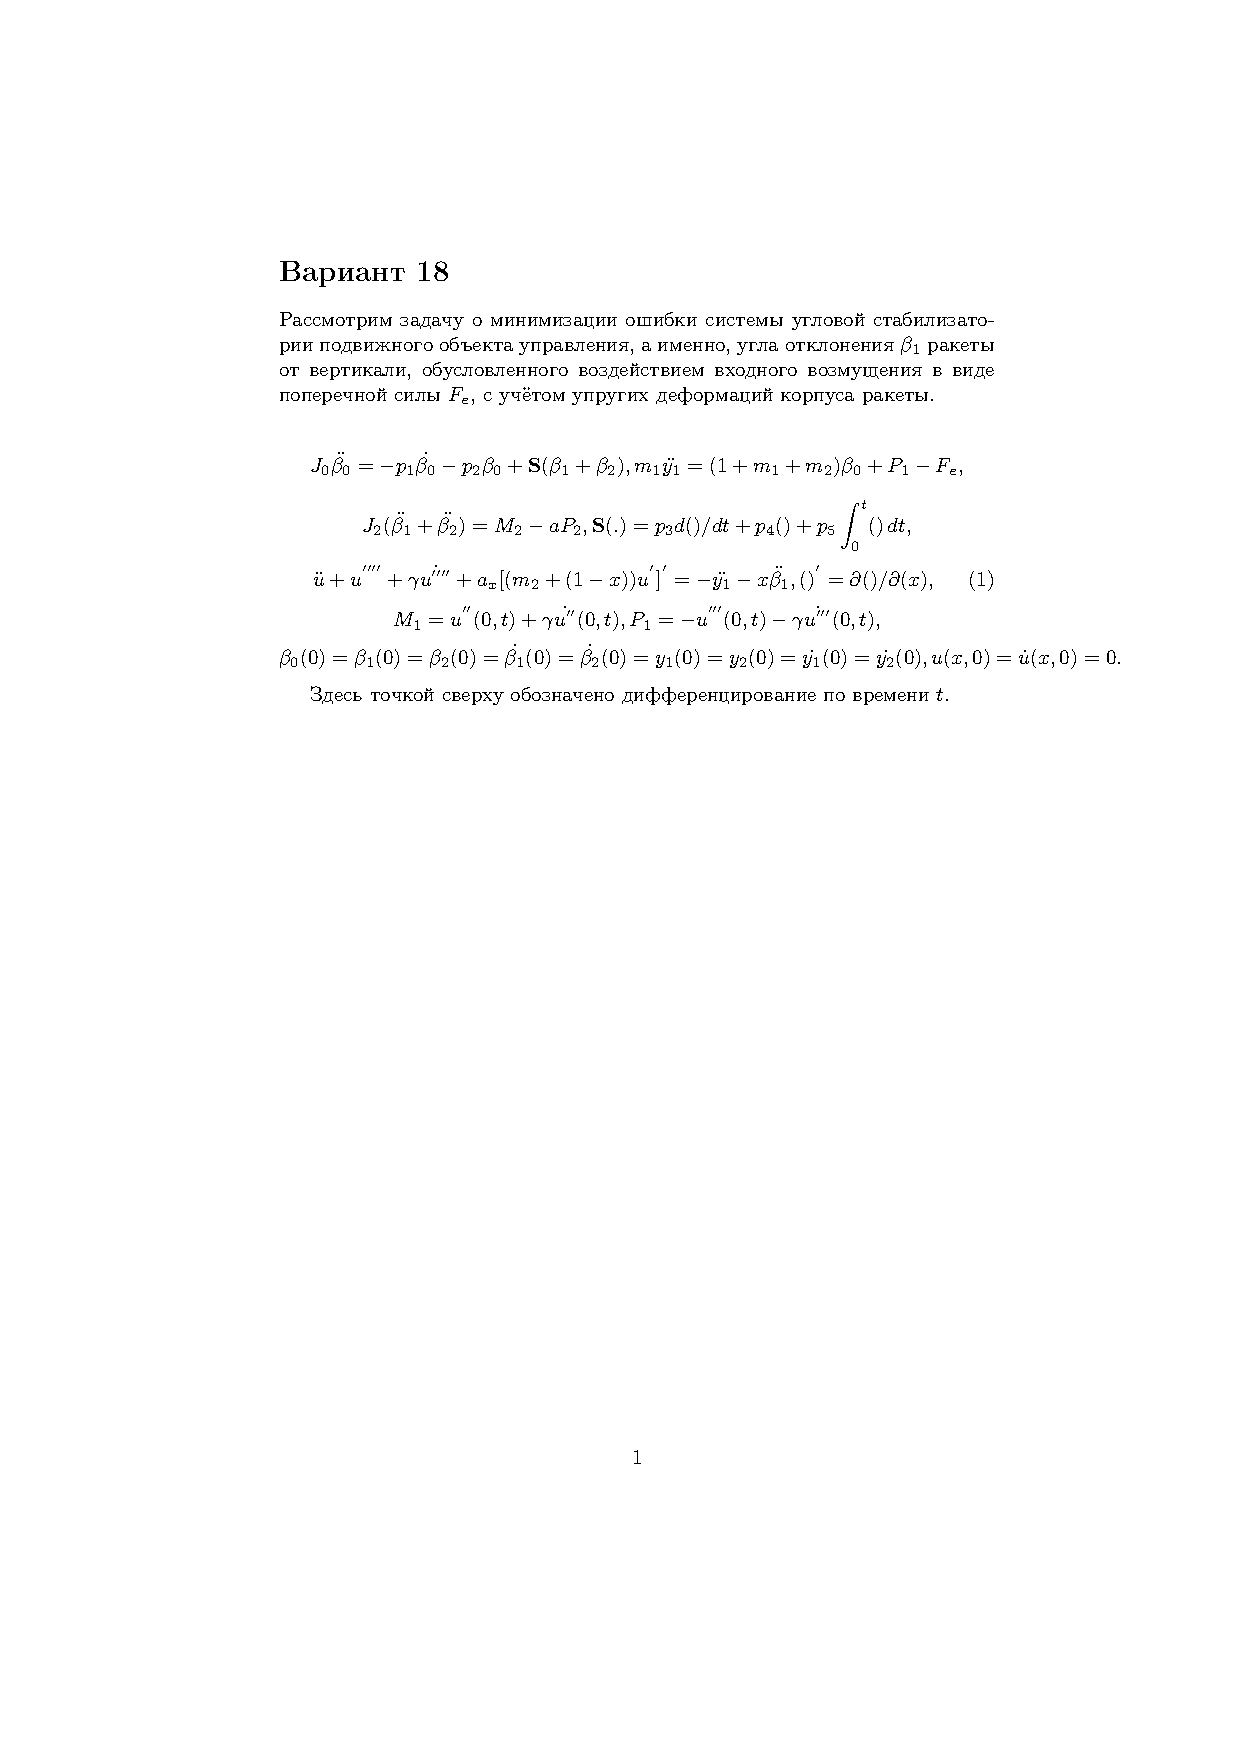
\includegraphics[width = \textwidth]{3.gif}
        
        \caption{Схематическое изображение малого правого вращения}
    \end{figure}

    Данное вращение используется тогда,
    когда (высота $b$"=поддерева "--- высота $R$)
    $= 2$ и высота $С \leqslant $ высоты $L$.
\end{frame}